\documentclass[10pt, a4paper]{article}
\usepackage[left=2cm, right=2cm, top=2cm]{geometry}
\usepackage[utf8]{inputenc}
\usepackage{amsmath}
\usepackage{amsfonts}
\usepackage{amssymb}
\usepackage{amsthm}
\usepackage{mathptmx}

\usepackage{float}
\usepackage{subfigure}
\usepackage{framed}
\usepackage{graphicx}
\graphicspath{{images/}}


% APA citation style
\usepackage{apacite}

\title{Sequence learning and recall in recurrent neural networks with time filtered units.}
\author{Ram\'on H. Mart\'inez-Mayorquin $^1$, Anders Lansner and $^1$ Pawel Herman $^1$
%
% Optional short acknowledgment: remove next line if non-needed
% \thanks{This is an optional funding source acknowledgement.}
%
% DO NOT MODIFY THE FOLLOWING '\vspace' ARGUMENT
\vspace{.3cm}\\
%
% Addresses and institutions (remove "1- " in case of a single institution)
1- KTH Royal Institute of Technology \\
Department of Computational Science and Technology - Stockholm, Sweden.
%
% Remove the next three lines in case of a single institution
\vspace{.3cm}\\ 
}

\setlength{\parskip}{0.3cm}
\begin{document}
\maketitle

There is a growing interest in studying the capability to learn, store and flexibly recall sequential patterns in neural network models. Processing sequential information bears particular relevance to a wide scope of cognitive functionality and behavior in humans \cite{lashley1951problem}. Hebb proposed that sequential activation of neural cell assemblies, referred to as phases sequences, form the basis of the human thought process \cite{hebb2005organization}. Serial order can be attributed to speech perception and generation, motor control and planning as well as goal directed behavior orchestrated by working memory. Therefore the question as to how a novel sequence of items is stored and recalled in the corrected order has been extensively studied in the context of memory systems among others. Besides intensive efforts in this direction undertaken in the domain of cognitive neuroscience and psychology \cite{hurlstone2014memory} the problem of sequence learning has also attracted a lot of theoretical interest. It has resulted in the development of different computational network models simulating the brain's capabilities to process sequence information. A prominent share of this computaitonal endevaour is linked to spiking neural network approaches to learn precise patterns of spike sequences with biologically plausible local learning rules \cite{ans1994neural}\cite{dehaene1987neural}\cite{gutig2006tempotron}\cite{ponulak2010supervised}. Another group of network approaches developed in the realm of rate based models offers a more generic context for sequence memory function \cite{amari1972learning}\cite{kohonen1977principle}\cite{sandberg2002bayesian}. 


The work presented here belongs to that category of connectionist based rate models and conceptually builds on \cite{sandberg2002bayesian}. As our main contribution we propose the use of a new Hebbian learning associative rule with synaptic gating \cite{andrew2003spiking} that provide a simple recurrent neural network with capabilities to learn and recall sequences of memory items. The proposed rate based model constitutes a well-controlled framework for studying the both learning and processing of sequences at the sub-symbolic level and identifying key parameters responsible for sequence processing capabilities in a dynamical connectionist system with all-to-all recurrent connectivity pattern. 


The recurrent neural network in Fig. \ref{Fig:diagrams} is composed of firing rate units with the input-output characteristics described by the logistic function $\Phi(x) = \frac{1}{1 + \exp(-Gx)}$ with gain G. The synaptic inputs are aggregated across the entire network through all-to-all connections weighted by synaptic weights $W$, and the activation of unit $U_i$, is then consistently determined by integrating synaptic inputs with the time constant $\tau_{m}$ (\ref{eq1}). To account for the temporal effect of synaptic smoothing we introduce the idea of z-filters  \cite{tully2016spike} that maintain the exponentially decaying traces of the activity with the time constant of $\tau_z$ (\ref{eq2}). This allows for keeping synaptic memory of the unit activity and influencing other post-synaptic units in the network even when the original pre-synaptic unit is not longer active. 

\begin{align}
\tau_m \dfrac{dx_i}{dt} &= \Phi\Big(\sum_{j} W_{ij} z_j - \theta \Big) - x_i \label{eq1} \\ 
\tau_z \dfrac{dz_i}{dt} &= x_i - z_i \label{eq2}
\end{align}



In this work we examine two types of learning rules, pre-synaptic (3) and post-synaptic (4)
gating \cite{andrew2003spiking}, which equip the proposed network with the capability to learn
how to recall sequential activity patterns.

\begin{align}
\tag{3 pre-synaptic}
\tau_w \dfrac{dw}{dt} &= (w_{max} - w) z_{pre}z_{post} + (w_{min} - w) (1 - z_{post})z_{pre} \label{eq:pre-synaptic rule}  \\
\tag{4 post-synaptic}
\tau_w \dfrac{dw}{dt} &= \underbrace{(w_{max} - w)}_{\text{saturation}} \underbrace{z_{pre}z_{post}}_{\text{Hebbian}} + \underbrace{(w_{min} - w)}_{\text{saturation}}\underbrace{ (1 - z_{pre})z_{post}}_{\text{synaptic-gating}} \label{eq:post-synaptic rule}
\end{align}

\begin{figure}[H]
\centering
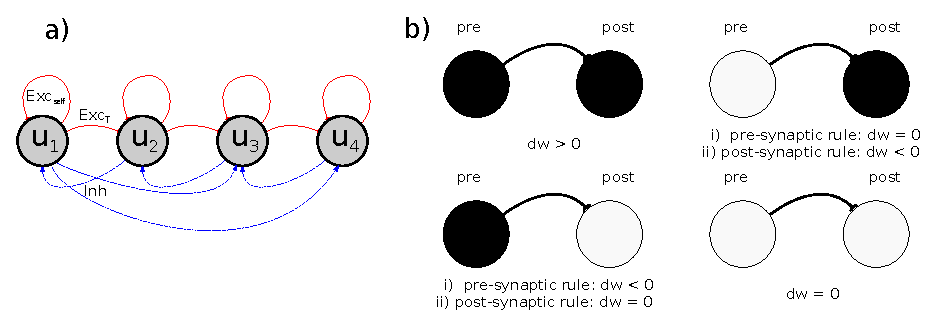
\includegraphics[scale=0.8]{diagram_mixed.eps}
\caption{a) Scheme of the overall network connectivity of the system. Note that the inhibitory connections are only fully depicted for the first unit for the sake of clarity. b) Conceptual illustration of the mechanism of learning induced synaptic changes. Here the a black filling stands for an active unit. } \label{Fig:diagrams}
\end{figure}


The first term in (\ref{eq:pre-synaptic rule}) and (\ref{eq:post-synaptic rule}) is an associative Hebbian contribution \cite{hebb2005organization} and its role is to strengthen the connections between activated units. Importantly however, in comparison with the original formulation \cite{andrew2003spiking}, we use the z-filters instead of the unit activities. This provides the scope for making associative connections between units even when either of the two units is no longer active provided that its memory trace is retainedby the synapse. As mentioned earlier, the synaptic trace decays exponentially with the time constant of $\tau_z$ (\ref{eq2}), and to preserve serial recall order we introduce asymmetrical time constants for z-pre and z-post : $\tau_{z_{pre}} > \tau_{z_{post}}$. The second term is called synaptic gating \cite{andrew2003spiking}, which facilitates the formation of inhibitory connections whenever the activity (or its z-filtered trace) of one unit is not accompanied with the activity of the other unit. We examine two variations of this term to explore the functional implications of both pre- and post-synaptic gating. Finally, the weights are kept between $w_{min}$ and $w_{max}$ limits. The nature of synaptic changes under the synaptic gating rule is illustrated in Fig. \ref{Fig:diagrams}.


Our learning protocol consists in fixing (clamping) each unit of the sequence in succession for a given amount of time (training time). We perform this process an epochs number of times. It is important to note that while learning there is a period of one second between each epoch or presentation that serves the purposes of avoiding self-interference.  


\begin{figure}[H]
\centering
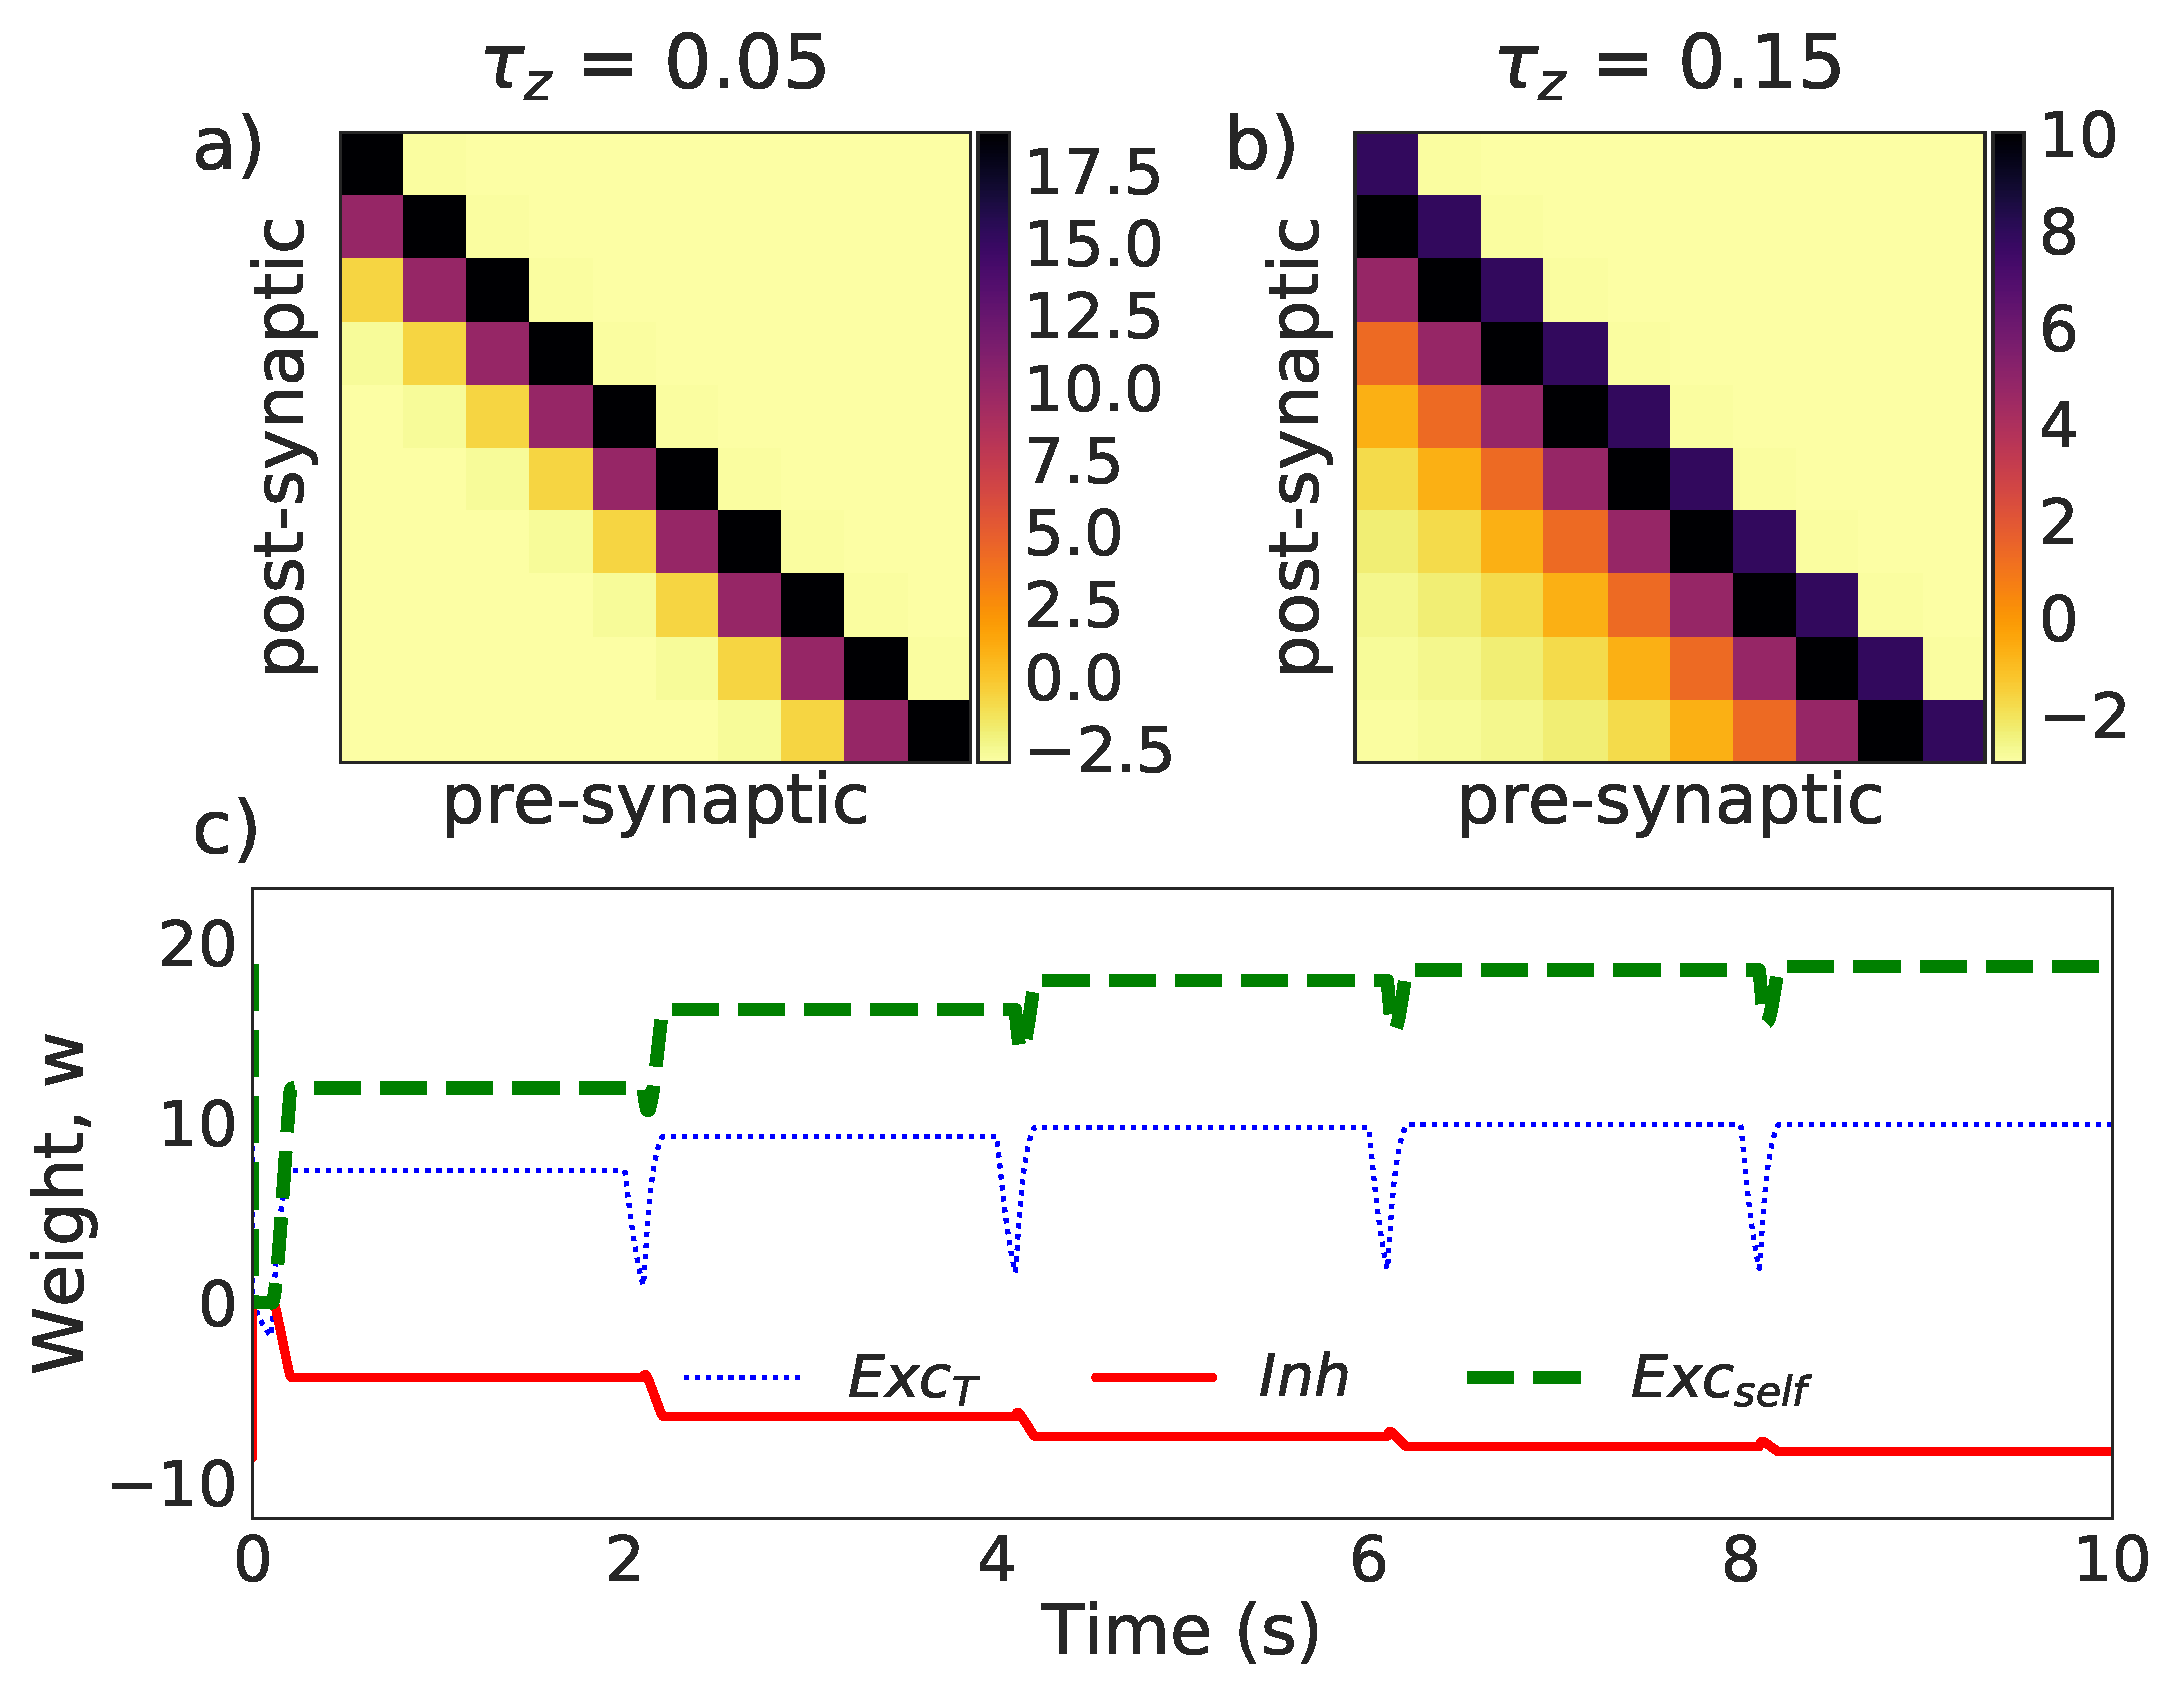
\includegraphics[scale=0.3]{training_rule.eps}
\caption{The effect of training with the learning rule. a) An example of training with a small value of $\tau_z=0.050s$. b) Same procedure as in a but with a longer time constant $\tau_z=0.150s$. c) evolution in time of the connection weights from the first to the second unit $Exc_T$, the one from the second back to the first unit $Inh$ and finally of the second unit into itself $Exc_{self}$. Five epochs of length $2s$ are shown here, note that this is enough time for the weights to stabilize.}\label{Fig:epochs}
\end{figure}

%\bibliographystyle{apacite}
\bibliographystyle{apacitex}
%\bibliographystyle{apacann}
%\bibliographystyle{apacannx}
%\bibliographystyle{apacite}
\bibliography{references.bib}
\end{document}

